%!TEX root=../../root.tex

\newpage

\section{Lezione 19}

\subsection{\texorpdfstring{$\overline{HAMPATH}$}{HAMPATH negato} \texorpdfstring{$\notin$}{non appartiene a} NP}

\begin{figure}[H]
    \centering
    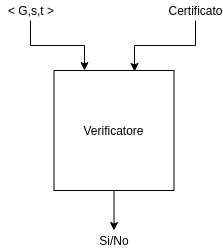
\includegraphics[scale=0.60]{notHam}
\end{figure}

\begin{gather*}
	\overline{HAMPATH} = \{ <G, s, t> \ | \ G \text{ è un grafo diretto senza cammini hamiltoniani} \\
	\text{da } s \text{ a } t \}
\end{gather*}
Il problema $\overline{HAMPATH}$ non è in $NP$ poiché non ammette un verificatore polinomiale, in quanto tale verificatore dovrebbe controllare che \textit{nessuna} permutazione di nodi sia un cammino hamiltoniano. Quindi il certificato da dare al verificatore dovrebbe necessariamente contenere tutte le possibili permutazioni dei vertici ed avere quindi tale dimensione (esponenziale), mentre nel caso di $HAMPATH$ era sufficiente fornire una possibile permutazione dei vertici come certificato.

\subsection{Relazione fra P e NP}

Uno dei maggiori problemi irrisolti dell'informatica teorica è quello di stabilire quale relazione lega $P$ ed $NP$, vi sono due possibilità:

\begin{figure}[H]
    \centering
    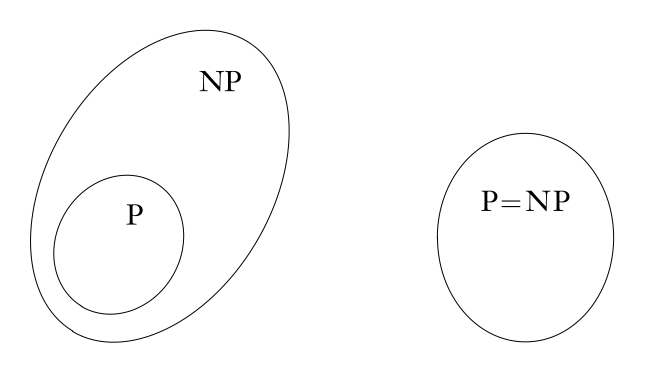
\includegraphics[scale=0.40]{PNP}
\end{figure}

Definiamo $ EXPTIME = \displaystyle \bigcup_{k \geq 0}{TIME(2^{O(n^k)})} $, 
sappiamo che $ NP \subseteq EXPTIME$ poiché si è visto che una $TM$ simula una $NTM$ con complessità di tempo $2^{O(t(n))}$, ma non sappiamo se esista una classe di complessità deterministica più piccola di $EXPTIME$ che contenga $NP$. 

Per dimostrare $P=NP$ si è cercato senza successo un metodo alternativo polinomiale per convertire una NTM in una TM deterministica, mentre per dimostrare $P\subsetneq NP$ si è cercato un problema in $NP$ con un limite inferiore non in $P$.


\subsection{Riduzione Polinomiale}

Un linguaggio $A$ si \textit{riduce polinomialmente} a un linguaggio $B$, ovvero in simboli $A \leq_p B$ se:
\[
   \exists \ f: \Sigma^{\star} \rightarrow \Sigma^{\star} \ \text{tale che}
\]
\begin{enumerate}
    \item \textit{f} è calcolabile in tempo polinomiale 
    \item $ x \in A \iff f(x) \in B $
\end{enumerate}

\subsection{I linguaggi CNFSAT e 3SAT}

\[
    CNFSAT = \{ \ \varphi \ | \ \varphi \in CNF \ \land \varphi \ \text{è soddisfacibile} \}
\]
Con $CNF$ si intende la Forma Normale Congiuntiva di una formula booleana, ovvero formata solo da \textit{clausole} in \textit{and}. Una clausola è un insieme di letterali in \textit{or}.

Si verifica facilmente l'appartenenza di CNFSAT ad NP esibendo un verificatore $V$:
\begin{description}
    \item \textit{input}: $<\varphi, s>$, con $\varphi \in CNF$ e $s \in \{0, 1\}^{\star}$ che rappresenta una assegnazione di verità ad ogni letterale (variabile o sua negazione) in $\varphi$

    \item \textit{descrizione}: verifica che ogni clausola valutata su tale assegnamento di letterali sia vera
\end{description}

Introduciamo ora il linguaggio $3SAT$, che in quanto sottoinsieme di $CNFSAT$, è in $NP$
\[
    3SAT = \{ \ \varphi \ | \ \varphi \in CNF  \text{ soddisfacibile } \land \text{ogni clausola è di 3 letterali} \}
\]

\paragraph{La riduzione}

\[
	\varphi = C_1 \land \dots \land C_k \text{ con } C_i \text{ clausola}
\]
Trasformiamo ogni clausola in una 3-clausola equivalente: sia 
\[
	C = X_1 \lor \dots \lor X_m
\] 
una generica clausola. La trasformazione è così descritta:

\begin{enumerate}
    \item $m=1$ \quad $C = X_1 \Rightarrow \varphi_C = X_1 \lor X_1 \lor X_1$
    \item $m=2$ \quad $C = X_1 \lor X_2 \Rightarrow \varphi_C = X_1 \lor X_2 \lor X_1$
    \item $m=3$ \quad C è già una 3-clausola
    \item $m\geq 4$
\begin{gather*}
	\varphi_C = \left( X_1 \lor X_2 \lor Z_1 \right) \land
		\left( \overline{Z_1} \lor X_3 \lor Z_2 \right) \land \dots \land
        \left( \overline{Z_{i-2}} \lor X_i \lor Z_{i-1} \right) \\
        \land \dots \land \left( \overline{Z_{m-3}} \lor X_{m-1} \lor X_{m} \right)
\end{gather*}
\end{enumerate}

Nei primi tre casi è ovvio che $C \text{ soddisfacibile} \Rightarrow \varphi_C$ soddisfacibile; nel quarto caso un po' meno, e lo mostreremo esplicitamente.

\subparagraph{C è soddisfatta $\Rightarrow \varphi_C$ è soddisfatta}
$$C \ \text{soddisfatta} \Rightarrow \ \exists \ i \ | \ X_i=1, \ 1\leq i \leq m$$
\begin{align}
 & i = 1,2  & & \Rightarrow Z_j = 0 & \forall \ 1\leq j \leq m-3  \\
 & i = m-1,m & & \Rightarrow Z_j = 1  & \forall \ 1\leq j \leq m-3 \\
 & 2 < i < m-1 &  & \Rightarrow Z_j = 1  & \forall  \ 1 \leq j \leq i-2 \\  
 & & & \text{e} \ \ \ Z_j = 0 &  \forall \ \ i-1\leq j \leq m-3 \nonumber
\end{align}
Se $X_1$ o $X_2$ sono vere, allora la prima clausola è vera: costruire una $\varphi_C$ con tutte le $Z_j = 0$ fa sì che tutte le clausole intermedie siano vere, in quanto contengono la negazione di una qualche $Z_k$, e così anche l'ultima che contiene $\overline{Z_{m-3}}$.

Se $X_{m-1}$ o $X_m$ sono vere, allora l'ultima clausola è vera: costruire una $\varphi_C$ con tutte le $Z_j = 1$ fa sì che tutte le clausole intermedie siano vere, similmente a prima, e così anche la prima che contiene $Z_1$.

Se infine è l'assegnamento di una qualche $X_i$ intermedia a rendere soddisfatta $C$, allora l'$i$-esima clausola è vera, e bisogna far sì che lo siano anche tutte le altre. Costruendo $\varphi_C$ con $Z_j = 1$ fino a $j = i-2$, le clausole precedenti sono sicuramente vere, in quanto ogni clausola (inclusa la prima) contiene un letterale vero; se $Z_j = 0$ da $j=i-1$ in poi, le clausole successive sono sicuramente vere, in quanto ogni clausola (inclusa l'ultima) contiene un letterale che è la negazione di una variabile falsa.

\subparagraph{$\varphi_C$ soddisfatta $\Rightarrow C$ soddisfatta}
\quad
Supponiamo per assurdo che C non sia soddisfatta dall'assegnamento che rende vera $\varphi_C$, cioè $X_i = 0 \quad \forall \ 1 \leq i \leq m$.

Se $X_i = 0 $ allora a rendere vere le clausole di $\varphi_C$ dovrebbero essere le $Z_i$: se fosse $Z_i = 1$ per ogni $i$, allora l'ultima clausola sarebbe falsa; se fosse $Z_i = 0$ per ogni $i$, allora la prima clausola sarebbe falsa; in generale qualunque fosse l'assegnamento delle $Z_i$, ci sarebbe almeno una clausola di $\varphi_C$ falsa, e quindi $\varphi_C$ non sarebbe soddisfatta in contraddizione con l'ipotesi.

\subsection{Teorema di Cook-Levin}

\paragraph{NP-completezza}
Un linguaggio $A$ è detto $NP$-completo se soddisfa due condizioni:
\begin{enumerate}
    \item $\forall B \in NP$, $B \leq_{p} A$ (A è NP hard)
    \item $A \in NP$
\end{enumerate}
Cook e Levin introdussero il concetto di \textit{NP-completezza}, ovvero la proprietà di un linguaggio per cui qualsiasi altro linguaggio in $NP$ si può ridurre polinomialmente ad esso. Essi dimostrarono che $SAT$ (e in particolare $CNFSAT$) è $NP$-completo, con una dimostrazione che non vediamo in quanto lunga, poiché deve prendere in esame un linguaggio $L$ generico e mostrare che $L \leq_p SAT$.

\paragraph{Transitività della riduzione} $A \leq_p B \leq_p C \implies A \leq_p C$

\subparagraph{Dimostrazione}
Sia $f$ la funzione di riduzione per $A \leq_p B$ e $T_f$ una $TM$ che la calcola in tempo polinomiale $O(n^k)$. 

Sia inoltre $g$ la funzione di riduzione per $B \leq_p C$ e $T_g$ una $TM$ che la calcola in tempo polinomiale $O(n^{k'})$.

Allora è possibile comporre $T_f$ e $T_g$ ottenendo una $TM$ che, dato un $x \in A$, calcola $g(f(x)) \in C$ in un tempo polinomiale $O((n^k)^{k'}) = O(n^{k \cdot k'}) = O(n^{k''})$.

Grazie a questa proprietà, per mostrare che un linguaggio è $NP$-hard basta mostrare che sia possibile ridurre polinomialmente $CNFSAT$ ad esso. Infatti se $CNFSAT \leq_p A$, allora significa che per qualunque $B \in NP$ vale $B \leq_p CNFSAT \leq_p A$, ovvero $B \leq_p A$ ovvero $A$ è $NP$-hard. Se si sa che $A \in NP$, allora $A$ è anche $NP$-completo. Ad esempio, abbiamo mostrato che $CNFSAT \leq_p 3SAT$, e poiché $3SAT \in NP$, possiamo affermare che $3SAT$ è $NP$-completo.

\paragraph{Lemma}
Se un linguaggio è riducibile polinomialmente a un linguaggio in $P$, allora anche esso è in $P$.
\[
        B \in P \land A \leq_{p} B \implies A \in P
\]

\paragraph{Enunciato} 
\[
B \text{ è } NP\text{-completo } \land B \in P \implies P = NP
\]
\paragraph{Dimostrazione}

Se $B$ è $NP$-completo allora ogni altro linguaggio $A \in NP$ si riduce polinomialmente ad esso. Ma $B \in P$, allora per il lemma precedente qualsiasi $A$ che si riduce polinomialmente a $B$ è anch'esso in $P$. Dunque tutti i linguaggi in $NP$ stanno anche in $P$, dimostrando che $NP \subseteq P$, ovvero l'inclusione mancante per dimostrare $P = NP$.

\subsection{Esempi di riduzioni polinomiali}
\subsubsection{Clique}
\[
	CLIQUE(k) = \{ <G,s,t> \ \mid \ \text{G ha un clique di k-elementi} \}
\]	
Per affermare che $CLIQUE(k)$ sia $NP$-completo bisogna mostrare che:
\begin{enumerate}
    \item CLIQUE(k) $\in$ NP (vedi 18.3.2)
    \item 3SAT $\leq_{p}$ CLIQUE 
\end{enumerate}
Dobbiamo quindi esibire una $f$ di riduzione, calcolabile polinomialmente, tale che:
\[
	\varphi \xmapsto{f} <G,k> \text{ tale che } \varphi \text{ è soddisfacibile } \iff G_{\varphi} \text{ ha un clique di k-elementi}
\]

La $f$ costruisce il grafo $G$ nel seguente modo:
\begin{itemize}
	\item ogni nodo nel grafo corrisponde a un letterale presente nelle clausole di $\varphi$

	\item i nodi corrispondenti a letterali nella stessa clausola non sono connessi

	\item i nodi corrispondenti a letterali contraddittori non sono connessi

	\item tutti gli altri nodi sono connessi
\end{itemize}

\paragraph{Esempio}

\[
    \varphi = (X_1 \lor X_1 \lor X_2) \land (\overline{X_1} \lor \overline{X_2} \lor \overline{X_2}) \land (\overline{X_1} \lor X_2 \lor X_2)
\]
e il grafo che costruiamo è il seguente
\begin{figure}[H]
  \centering
  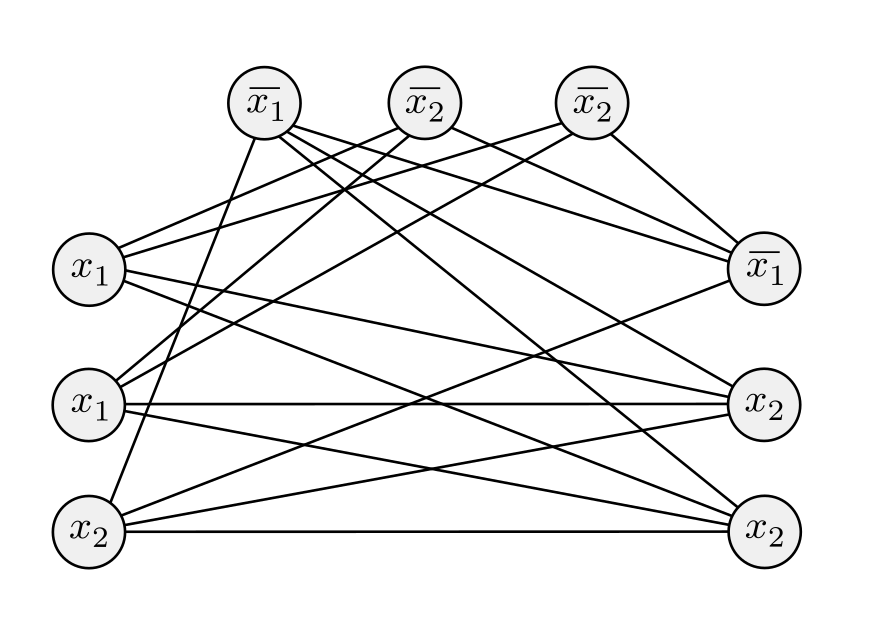
\includegraphics[scale=0.35]{GrafoClique}
\end{figure}

\paragraph{$\varphi$ soddisfacibile $\Rightarrow G_{\varphi}$ ha un $k$-clique}

Se $\varphi$ è soddisfacibile, e  $\varphi = C_1 \ \land \ C_2 \ \land$ \\
$\land \dots \land \ C_n$, allora essa ha un qualche assegnamento di verità che la rende soddisfatta. Consideriamo tale assegnamento: in ogni $C_i$ vi è almeno un letterale vero, che indichiamo con $X_i$. Costruiamo $G_{\varphi}$ con la regola di cui sopra e consideriamo i nodi etichettati con i vari $X_i$: essi sono $k$, tanti quante le clausole, e inoltre sicuramente sono connessi tra loro poiché, considerati a coppie
\begin{enumerate}
	\item non appartengono alla stessa clausola $C_i$

	\item non sono contraddittori, poiché se lo fossero allora o uno dei due non sarebbe vero (contraddizione), oppure $\varphi$ sarebbe contraddittoria (contraddizione)
\end{enumerate}
Quindi il sottografo formato dai nodi etichettati con i vari $X_i$ è una $k$-clique.

\paragraph{$G_{\varphi}$ ha un $k$-clique $\Rightarrow \varphi$ è soddisfacibile}
Se $G_{\varphi}$ ha un $k$-clique, nessun nodo nel clique corrisponde a letterali appartenenti alla stessa clausola, in quanto per costruzione essi non sono connessi. Di conseguenza ogni clausola contiene esattamente 1 letterale corrispondente a un nodo nel clique, perciò basta trovare un assegnamento di verità che rende vero ognuno di questi letterali per rendere soddisfatta $\varphi$. 

Tale assegnamento esiste sicuramente, in quanto i letterali del clique non sono contraddittori, altrimenti per costruzione non sarebbero connessi, e quindi non potrebbero far parte del $k$-clique (contraddizione).

Quindi $\varphi$ è soddisfacibile.

\subsubsection{IndSet}
\[
	INDSET = \{ <G,k> \ \mid G\text{ ha un independet-set di k-elementi}\}
\]
Con \textit{independet-set} si indica un sottoinsieme $S$ di nodi di $G$ per cui $v, w \in S \implies \{v, w\} \notin E_G$. 

Mostriamo che $INDSET$ è $NP$-completo:
\begin{enumerate}
    \item INDSET $\in$ NP (si verifica facilmente)
    \item 3SAT $\leq_{p}$ INDSET
\end{enumerate}

Come al solito, dobbiamo esibire una $f$ di riduzione per cui:
\begin{gather*}
	\varphi \xmapsto{f} <G_{\varphi}, k> \text{ tale che} \\
	\varphi \text{ ha k clausole ed è soddisfatta } \iff G \text{ ha un independent-set di dimensione k}
\end{gather*}

La $f$ costruisce $G$ nel seguente modo:
\begin{itemize}
	\item ogni nodo nel grafo corrisponde a un letterale presente nelle clausole di $\varphi$

	\item i nodi corrispondenti a letterali nella stessa clausola sono connessi

	\item i nodi corrispondenti a letterali contraddittori sono connessi

	\item tutti gli altri nodi non sono connessi
\end{itemize}

\newpage

\paragraph{Esempio}
\begin{equation*}
    \varphi = (X_1 \lor \overline{X_2} \lor X_1) \land (X_2 \lor \overline{X_1} \lor X_3) \land (X_1 \lor X_2 \lor X_3)
\end{equation*}

\begin{figure}[H]
  \centering
  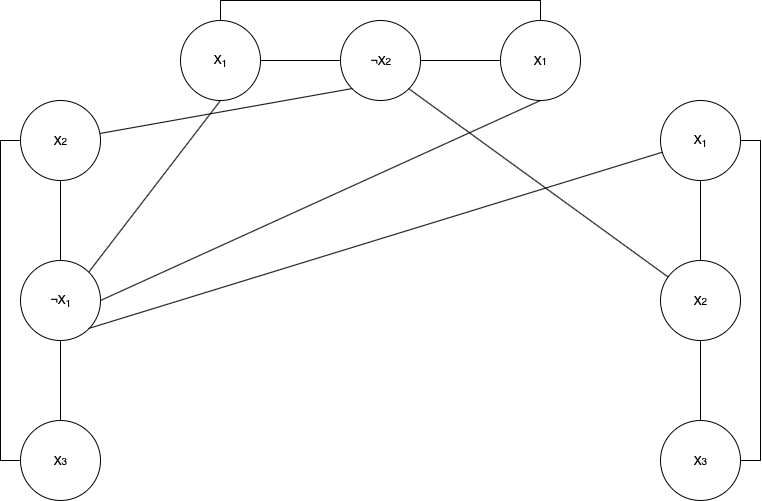
\includegraphics[scale=0.35]{IndSet}
\end{figure}

\paragraph{$\varphi$ soddisfacibile $\Rightarrow G_{\varphi}$ ha un independent-set di dimensione $k$}
Se $\varphi$ è soddisfacibile, e  $\varphi = C_1 \ \land \ C_2 \ \land \dots \land \ C_n$, allora essa ha un qualche assegnamento di verità che la rende soddisfatta. Consideriamo tale assegnamento: in ogni $C_i$ vi è almeno un letterale vero, che indichiamo con $X_i$. Costruiamo $G_{\varphi}$ con la regola di cui sopra e consideriamo i nodi etichettati con i vari $X_i$: essi sono $k$, tanti quante le clausole, e inoltre sicuramente \textit{non} sono connessi tra loro poiché, considerati a coppie
\begin{enumerate}
	\item non appartengono alla stessa clausola $C_i$

	\item non sono contraddittori, poiché se lo fossero allora o uno dei due non sarebbe vero (contraddizione), oppure $\varphi$ sarebbe contraddittoria (contraddizione)
\end{enumerate}
Quindi il sottografo formato dai nodi etichettati con i vari $X_i$ è un independent-set di dimensione $k$.

\paragraph{$G_{\varphi}$ ha un independent-set di dimensione $k$ $\Rightarrow \varphi$ è soddisfacibile}
Se $G_{\varphi}$ ha un independent-set di dimensione $k$, che chiamiamo $S$, allora nessun nodo in $S$ corrisponde a letterali appartenenti alla stessa clausola, in quanto per costruzione essi sono connessi. Di conseguenza ogni clausola contiene esattamente 1 letterale corrispondente a un nodo in $S$, perciò basta trovare un assegnamento di verità che rende vero ognuno di questi letterali per rendere soddisfatta $\varphi$. 

Tale assegnamento esiste sicuramente, in quanto i letterali in $S$ non sono contraddittori, altrimenti per costruzione sarebbero connessi, e quindi non potrebbero far parte di $S$ (contraddizione).

Quindi $\varphi$ è soddisfacibile.